\documentclass[12pt, a4paper]{report} %standard 12 punti, specifica anche la dimensione del documento
\usepackage[utf8]{inputenc} %specifica l'encoding
\usepackage{graphicx}
\usepackage{float}
\graphicspath{ {images/Final results/Architectures/Delays},{images/Final results/Architectures/Energy},{images/Final results/Architectures/Tasks}, {images} } %specifica il path al folder delle immagini
\usepackage[section]{placeins}
\usepackage{hyperref}
\hypersetup{
    colorlinks=true,
    linkcolor=blue,
    filecolor=magenta,      
    urlcolor=blue,
    pdftitle={Overleaf Example},
    pdfpagemode=FullScreen,
    }
%\counterwithin*{figure}{section} Posso resettare anche il contatore delle figure a ogni sezione
\counterwithin*{equation}{section} %Resetta il contatore delle equazioni a ogni sezione 
\counterwithin*{equation}{subsection}

\title{Report simulazione "Prima definizione"}
\author{Tommaso Lencioni}
%\date{} % Activate to display a given date or no date (if empty),
         % otherwise the current date is printed 

\begin{document}
\maketitle
Ho cercato di simulare una prima situazione di deployment di applicazioni su veicoli intelligenti usando architettura Cloud e Fog.\\
Dopo varie prove ho ottenuto i risultati presentati in questo report.
\section*{Infrastruttura}
\subsection*{Cloud}
Ho lasciato le specifiche del cloud invariate.\\
Ha due hosts ciascuno con con:
\begin{itemize}
	\item 8 core
	\item 2000000 mips
	\item 16 GB RAM
	\item 1000000 MB(?) di storage
\end{itemize}

\subsection*{Fog}
Il dispositivo edge datacenter simula una \textit{road side unit} (RSU).\\
Ho lasciato invariate le prestazioni dell'edge datacenter (2 hosts da 8 core, 800000 MIPS, 16GB RAM, 200000 MB(?) ciascuno) modificando solo la sua posizione (125 x, 125 y cioè al centro della mia simulazione)
\subsection*{Edge}
Ho utilizzato un solo tipo di device trattando un veicolo come un unico dispositivo impostando valori che rispecchiano il comportamento di un veicolo in un contesto urbano:

 \begin{itemize}
	\item L'architettura del processore è ARM.\footnote{ \url{https://www.arm.com/solutions/automotive}}
        \item È dotato di mobilità e di una velocità di 14 m/s (50 Km/h).
        \item I parametri di pausa e durata del movimento sono approssimativamente quelli di traffico scorrevole.
        \item Anche se non tutta l'energia è dedicabile al calcolo ho inserito come capacità della batteria quella della Nissan Leaf\footnote{\url{en.wikipedia.org/wiki/Nissan_Leaf}} (per fare gioco sull'efficienza questo numero adrebbe sicuramente ridotto)
	\item Come consumo massimo e in idle ho utilizzato i valori di circa 2 Raspberry Pi.
    \end{itemize}

\section*{Applicazioni}
Ho ipotizzato la presenza di 2 applicativi (originariamente solo 1, si vedano i \nameref{Dubbi}):

\begin{enumerate}
\item
	\begin{verbatim}
		SENSOR_DATA_COMMUNICATION
	\end{verbatim}
	Applicazione che simula la raccolta e comunicazione dei dati forniti dai sensori della vettura.\\
	\begin{itemize}
	\item Il rate è di 20, questo dovrebbe significare una chiamata ogni 3 secondi.
	\item Ho provato a settare l'user percentage a 100 (in quanto tutti i dispositivi hanno bisogno di comunicare dati) ma la simulazione non finiva di salvare le chart così ho deciso di diminuirla (questo sicuramente non è corretto ma non ho trovato un modo per ovviare al problema).
	\item La latenza massima permessa è di un secondo.
	\item Le dimensioni (container size 15000 KB, request size 100 KB, results size 500 KB e task lenght 10000 MI) sono indicative.\\
	Ho cercato di dare più peso alla risposta immaginandomi una situazione nella quale ricevo lo status della rete circostante.
	\item Ho lasciato il numero dei core richiesti a 1 (si vedano i \nameref{Dubbi}).
	\end{itemize}
	\item
	\begin{verbatim}
		ENTERTAINMENT
	\end{verbatim}
	Applicazione che simula l'utilizzo dell'infotainment di una vettura (musica streaming, webradio, etc)
	\begin{itemize}
		\item Il rate è di 10, questo dovrebbe significare una chiamata ogni 6 secondi.
		\item Per quanto riguarda l'user percentage stessa cosa di sopra.
		\item Il delay è di 5 secondi (ipotizzando che un contenuto audio sia traferito in una cache interna al device)
		\item La dimensione del Container è di 50MB.
		\item La richiesta è di 100KB e la risposta è di 40MB.
		\item La lunghezza del task è di 15000 MI.
		\item Per quanto riguarda i core stessa cosa di sopra.
	\end{itemize}
\end{enumerate}

\section*{Scenario}
Per questa simulazione ho previsto (riporto le modifiche sostanziali alla simulazione di default):
\begin{itemize}
	\item Una durata di 60 minuti.
	\item Una dimensione dell'area di simulazione di 250m$\times$250m.
	\item Il range degli edge devices di 50m
	\item il range degli edge datacenter di 180m (circa 125$\times\sqrt{2}$ così da inscrivere tutta l'area di simulazione essendo posizionato al centro)
	\item Il numero minimo di devices è 50 che crescono fino a 150 in scaglioni di 50.
	\item Ho utilizzato come architettura di orchestrazione CLOUD\_ONLY e MIST\_ONLY per fare un confronto.
	
\end{itemize}

\section*{Osservazioni}
Dai grafici ho tratti le seguenti conclusioni:
\begin{itemize}
	\item Il Cloud garantisce un delay di esecuzione minore rispetto all'offload su RSU (\autoref{fig.1}).
	\begin{figure}[!ht]
	\caption{Delay medio di esecuzione}
	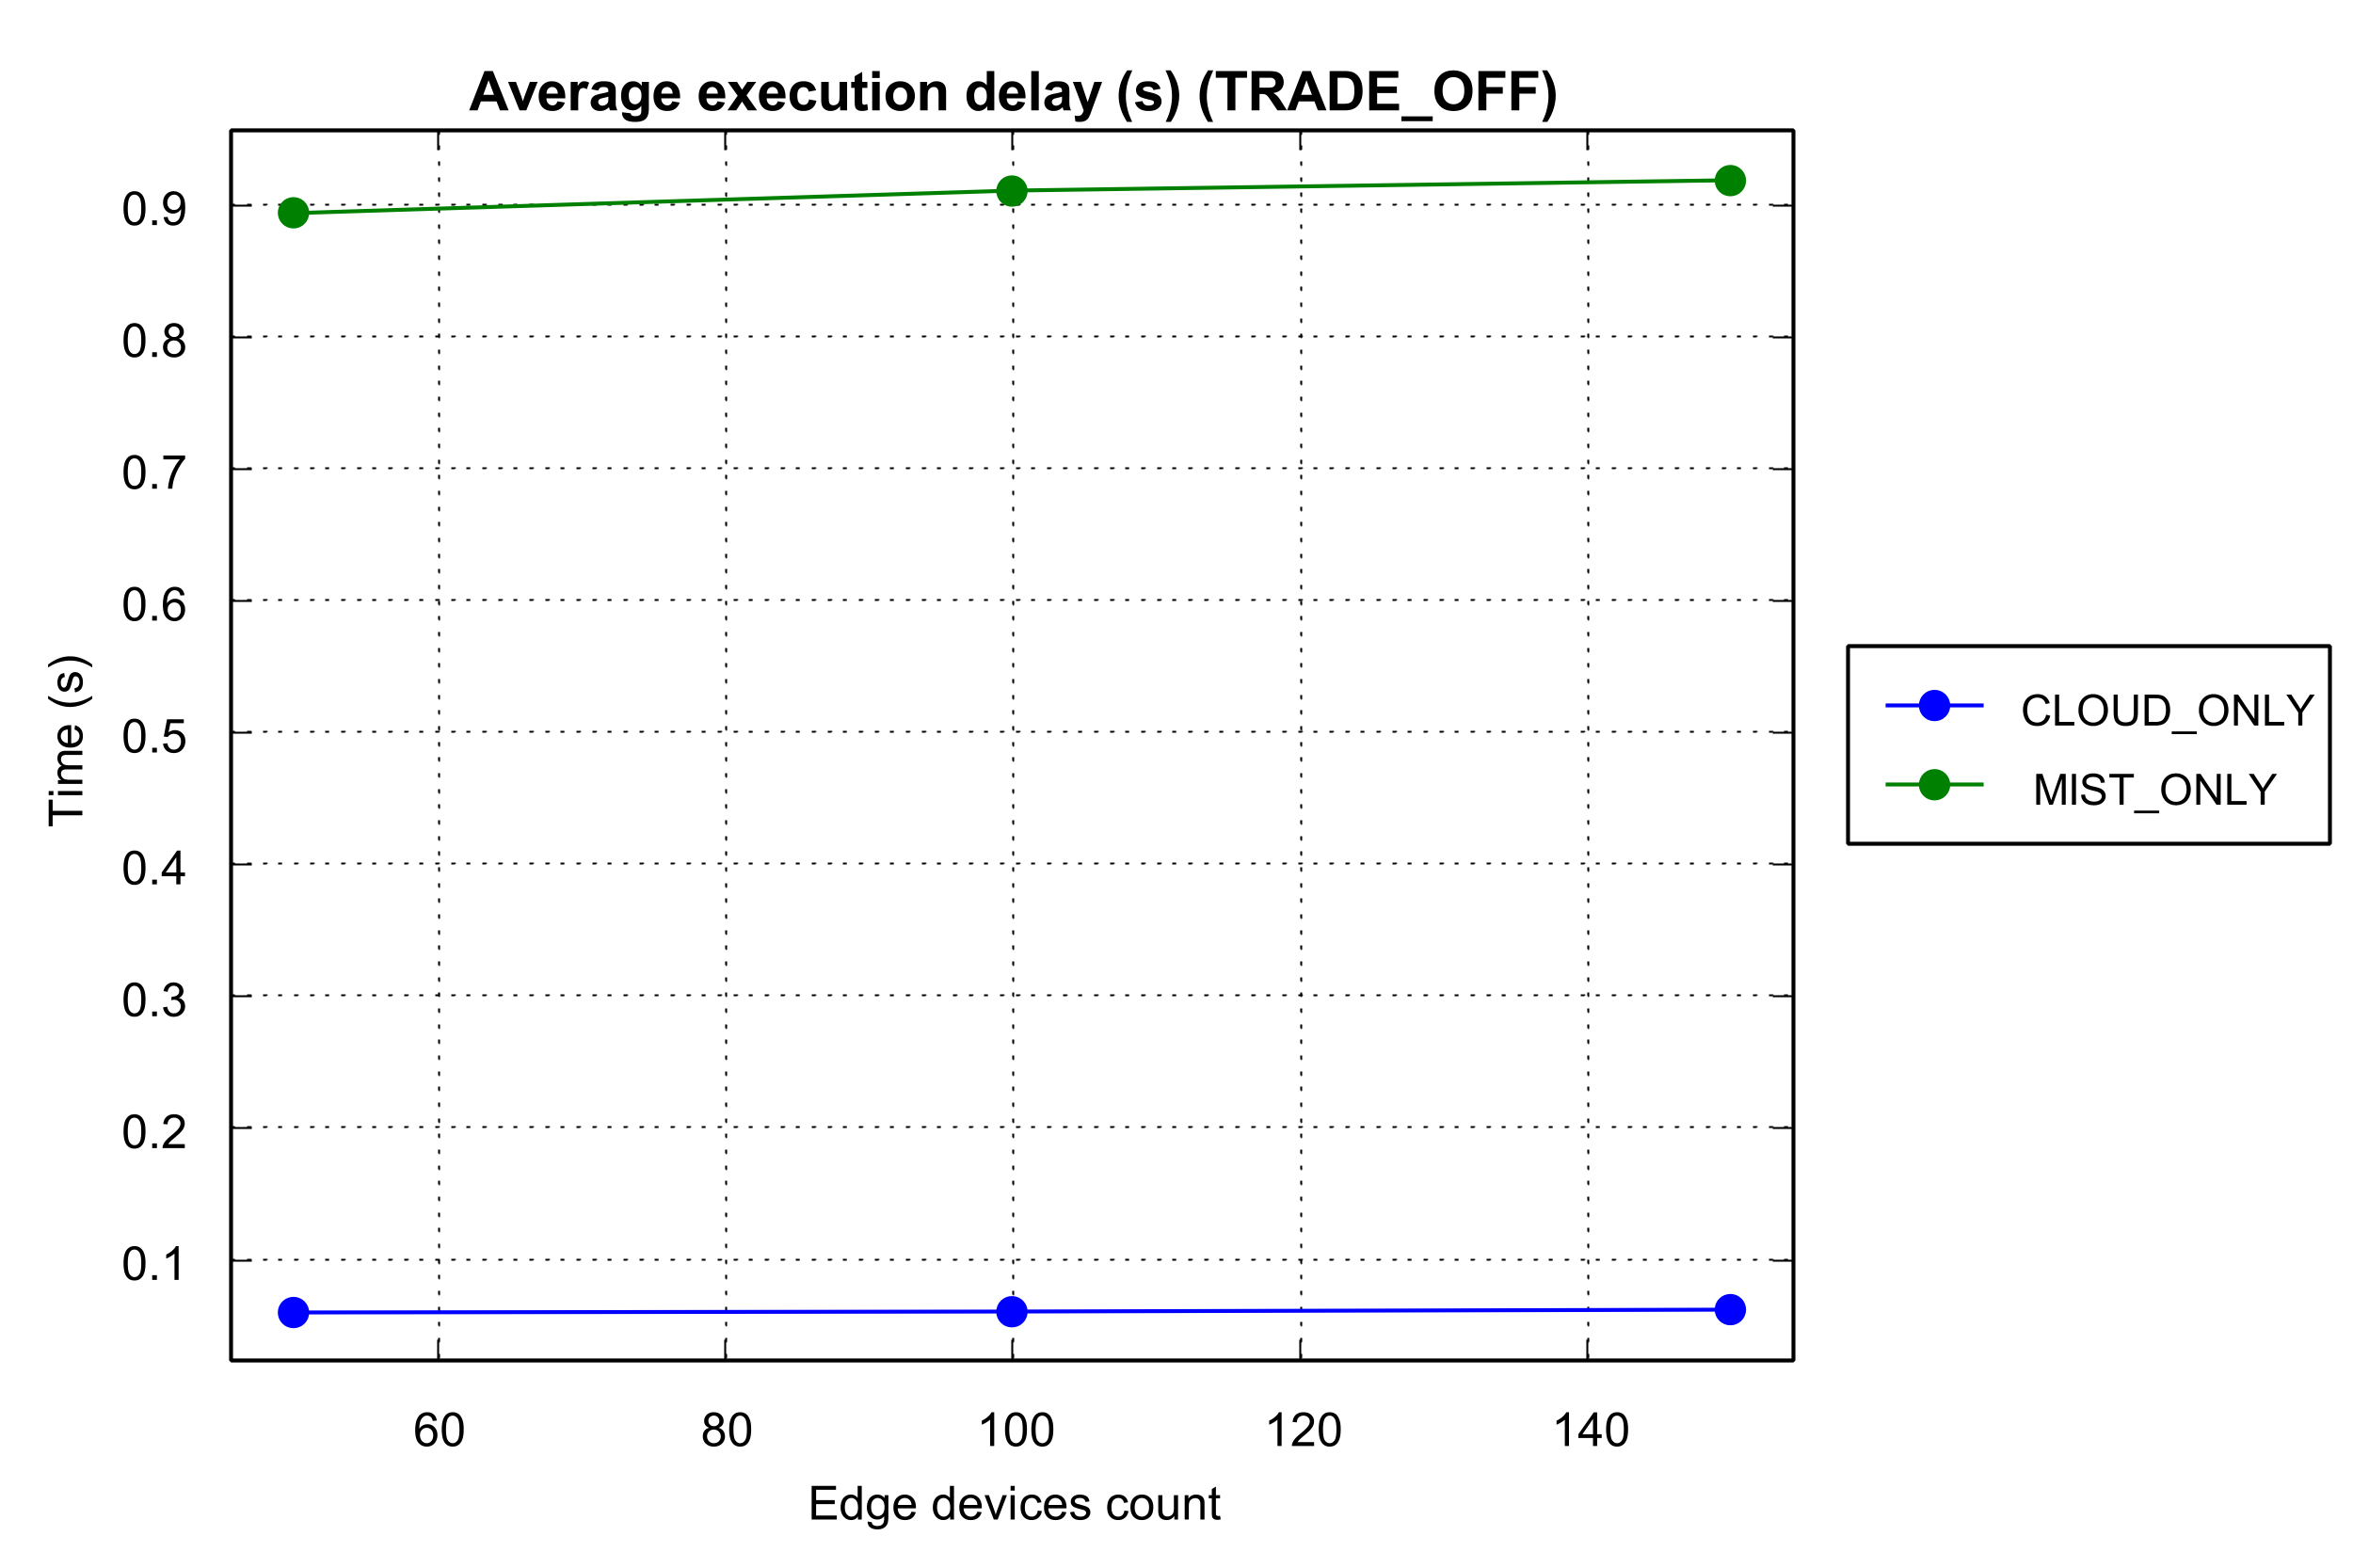
\includegraphics[scale=0.5]{Average execution delay (s)__TRADE_OFF}
	\centering
	\label{fig.1}
	\end{figure}
	\item  Nonostante le applicazioni vengano eseguite in meno tempo in Cloud il tempo di attesa è maggiore e, soprattutto, crescente  (\autoref{fig.2}).\\
	Ci possiamo aspettare che aumenti con l'aumento del numero dei devices fino a rendere nulla il vantaggio che ha il Cloud sull'execution delay.
	\begin{figure}[!ht]
		\caption{Tempo di attesa medio}
		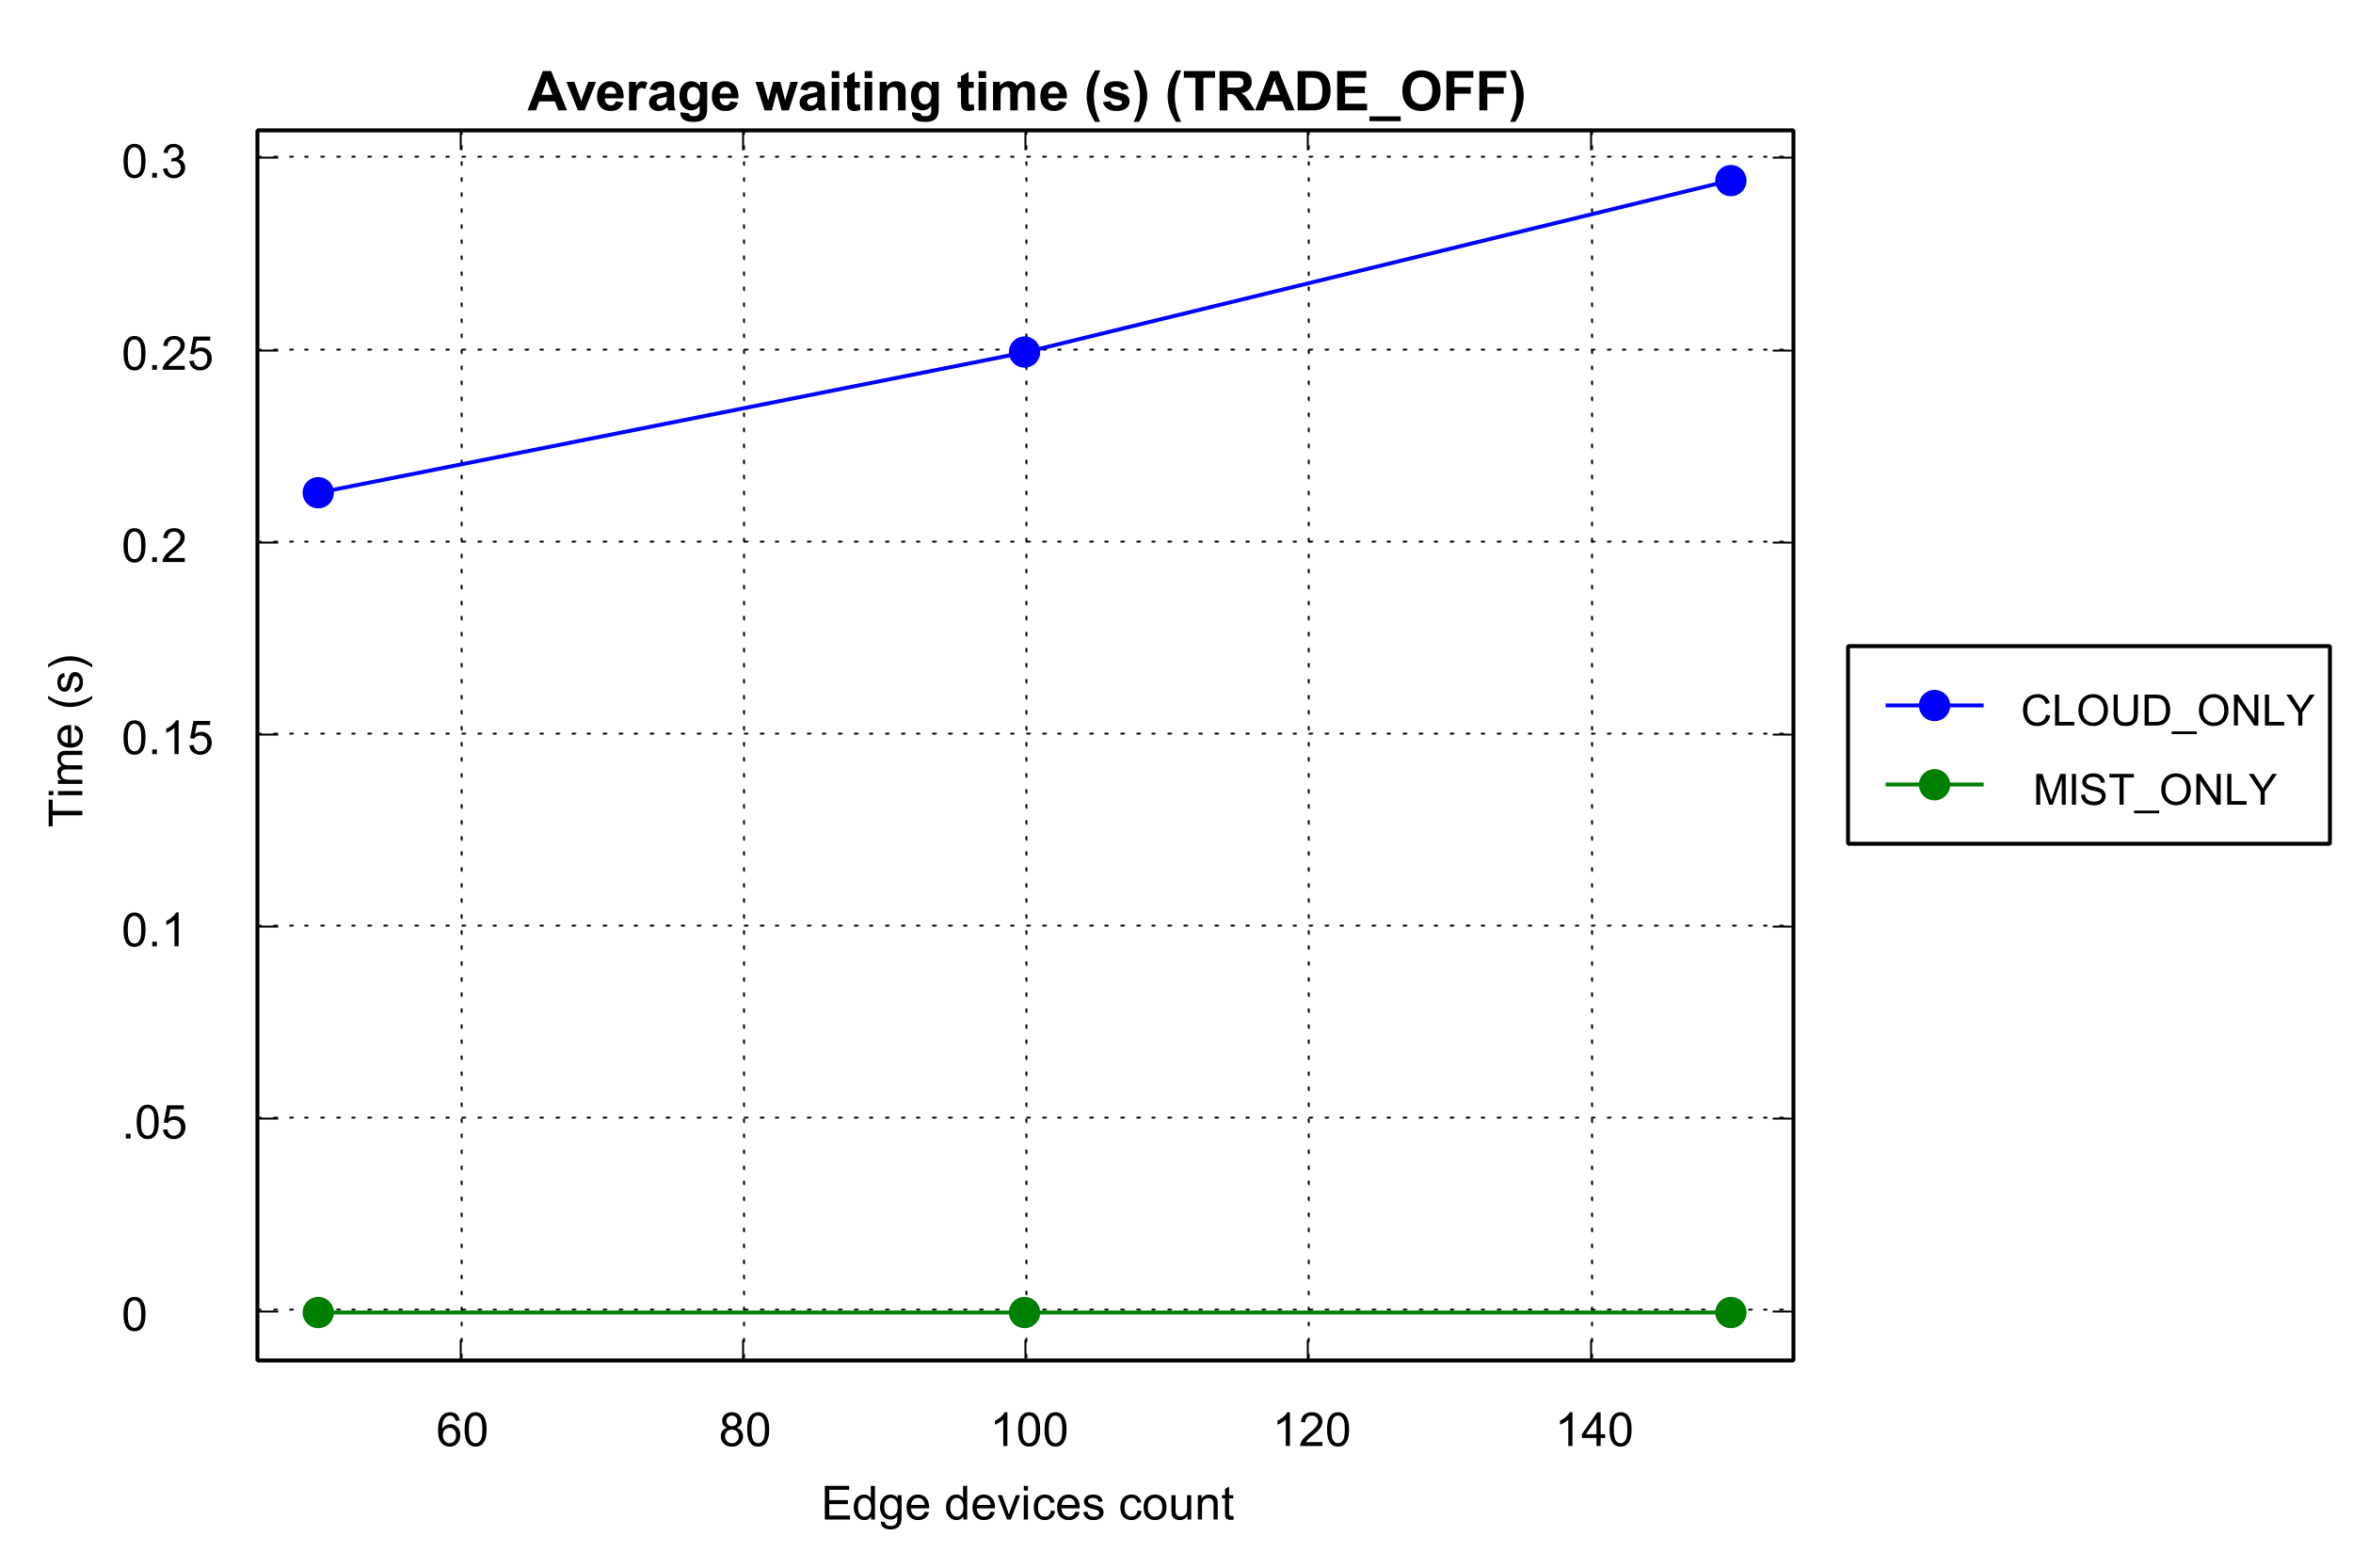
\includegraphics[scale=0.5]{Average waiting time (s)__TRADE_OFF}
		\centering
		\label{fig.2}
	\end{figure}
	\item  Il consumo di energia è inferiore per l'architettura Mist con una differenza crescente rispetto a Cloud (\autoref{fig.3}).
	\begin{figure}[!ht]
		\caption{Consumo di energia}
		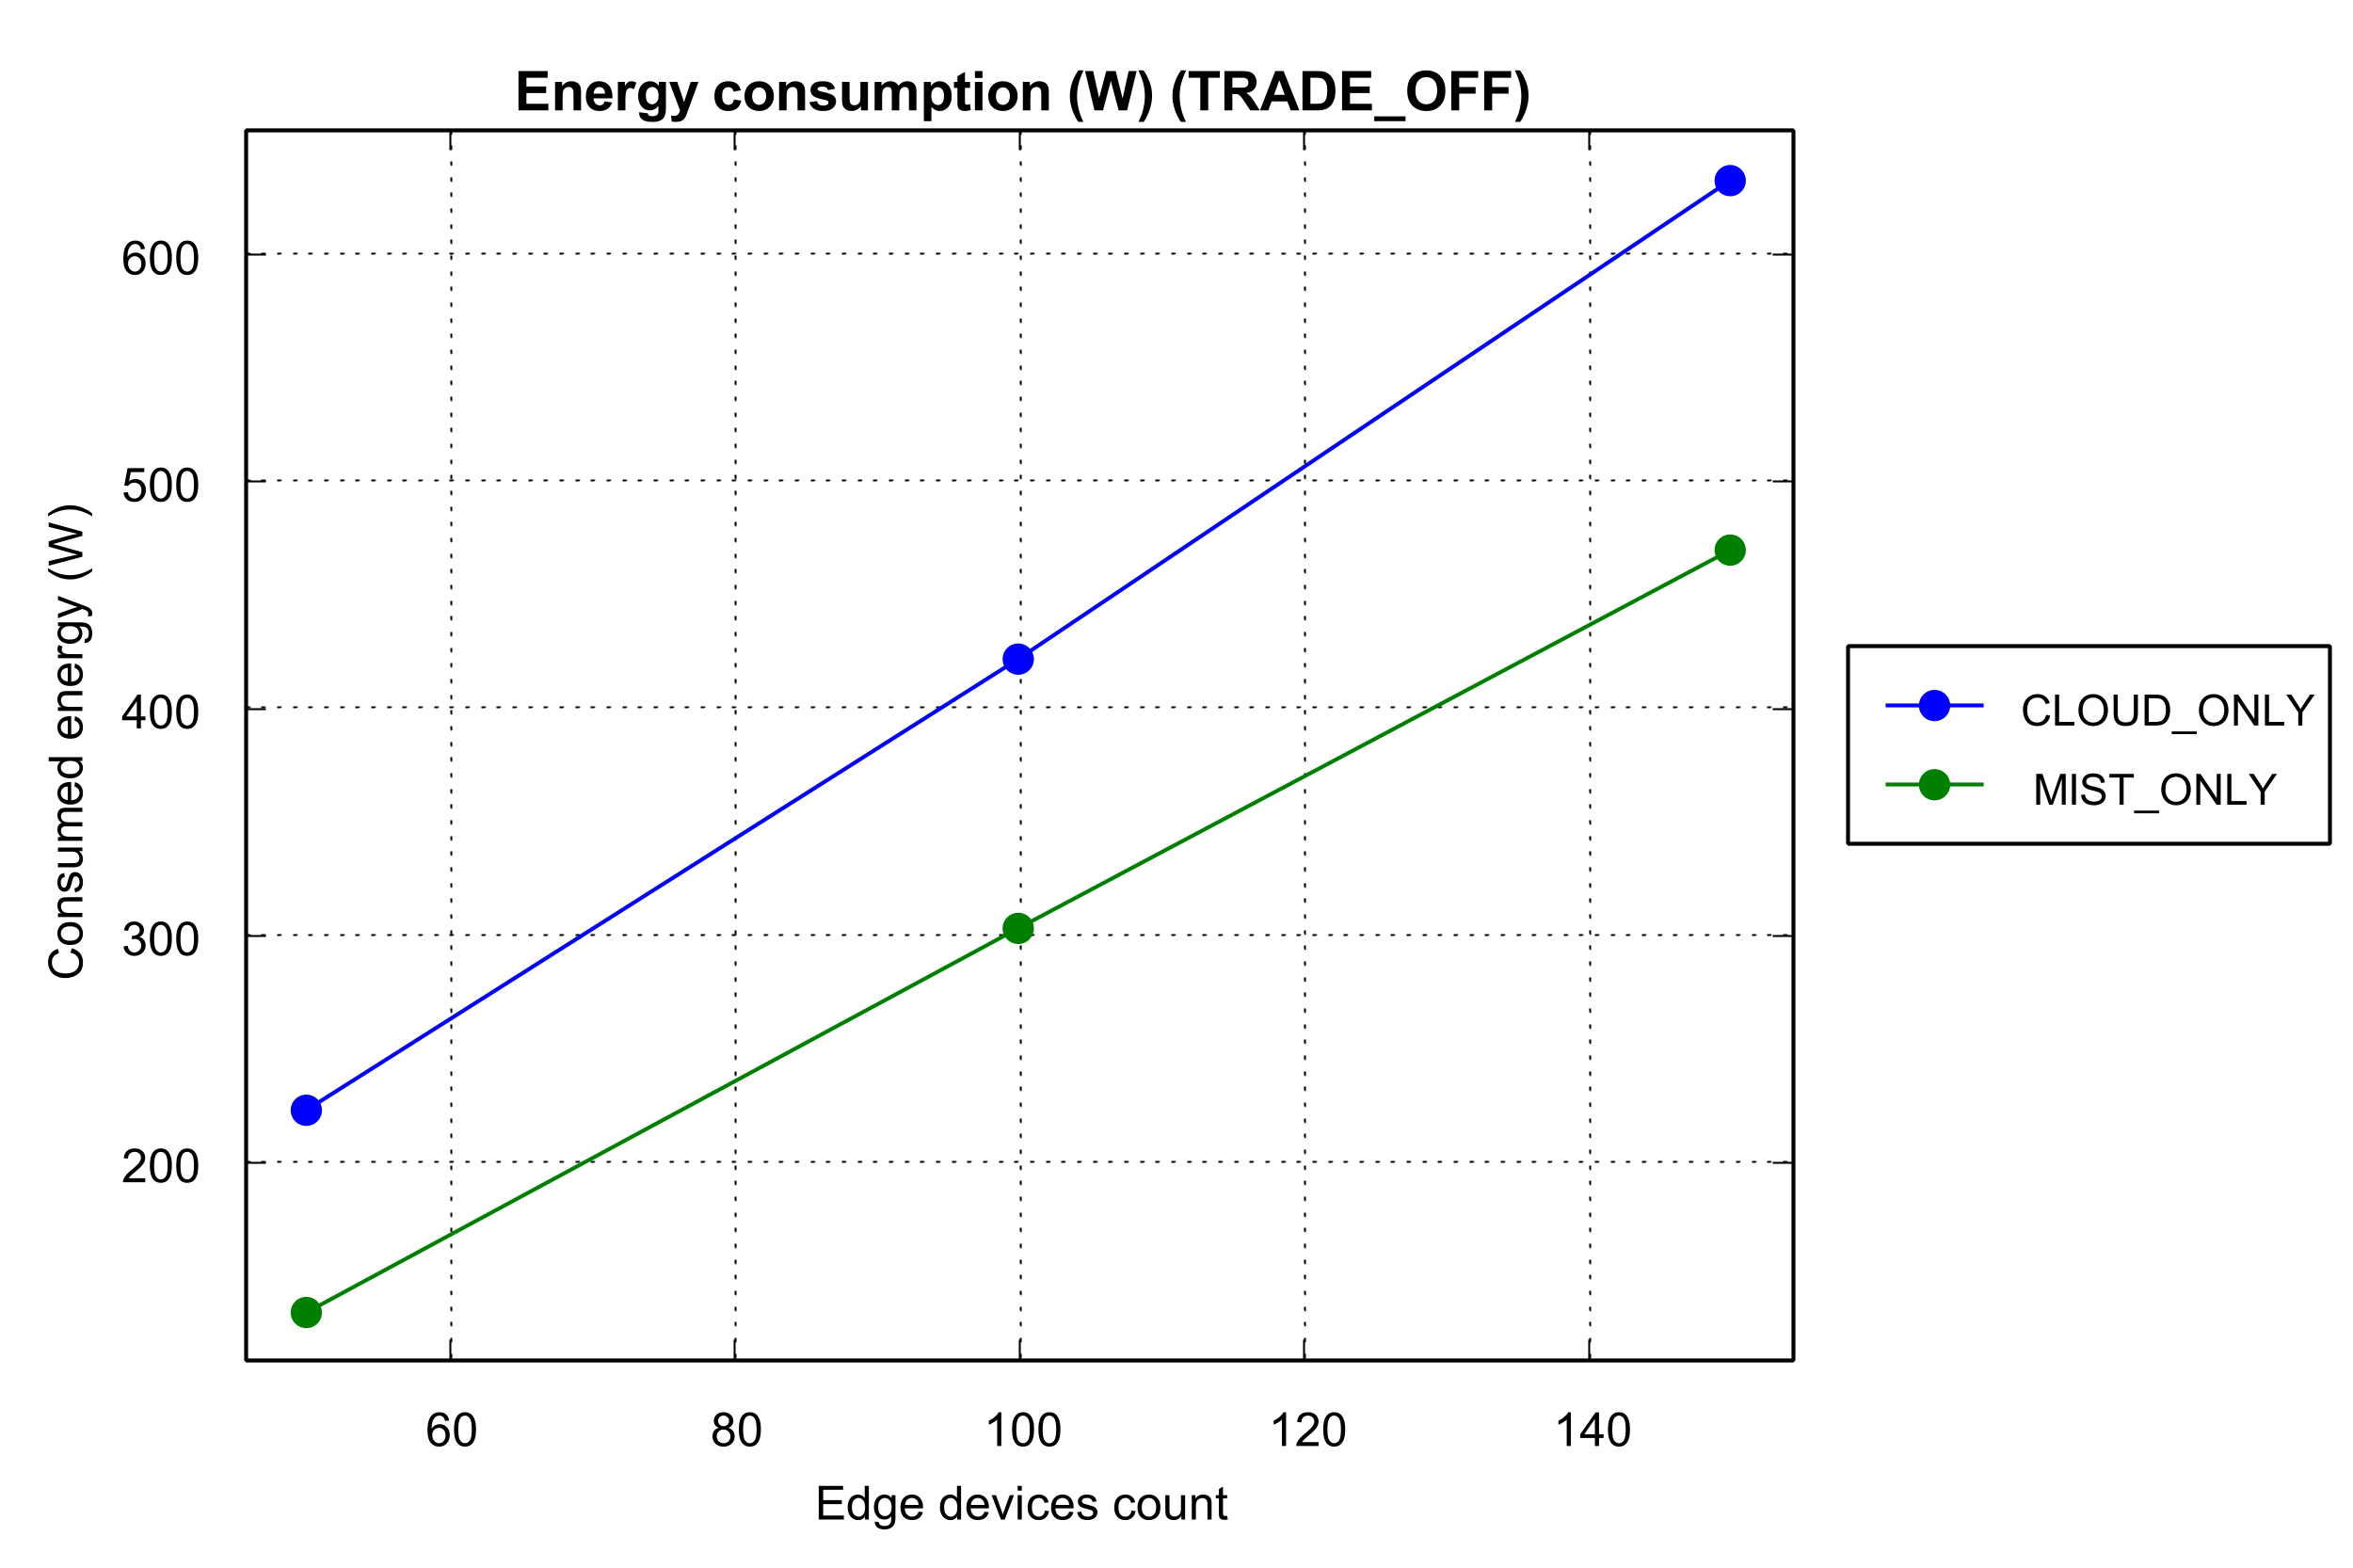
\includegraphics[scale=0.5]{Energy consumption (W)__TRADE_OFF}
		\centering
		\label{fig.3}
	\end{figure}
	\item  Il numero dei task falliti a causa del delay è maggiore nell'architettura Cloud (con crescita più rapida rispetto a Mist) (\autoref{fig.4}).
	\begin{figure}[!ht]
		\caption{Task falliti a causa dell'elevato delay}
		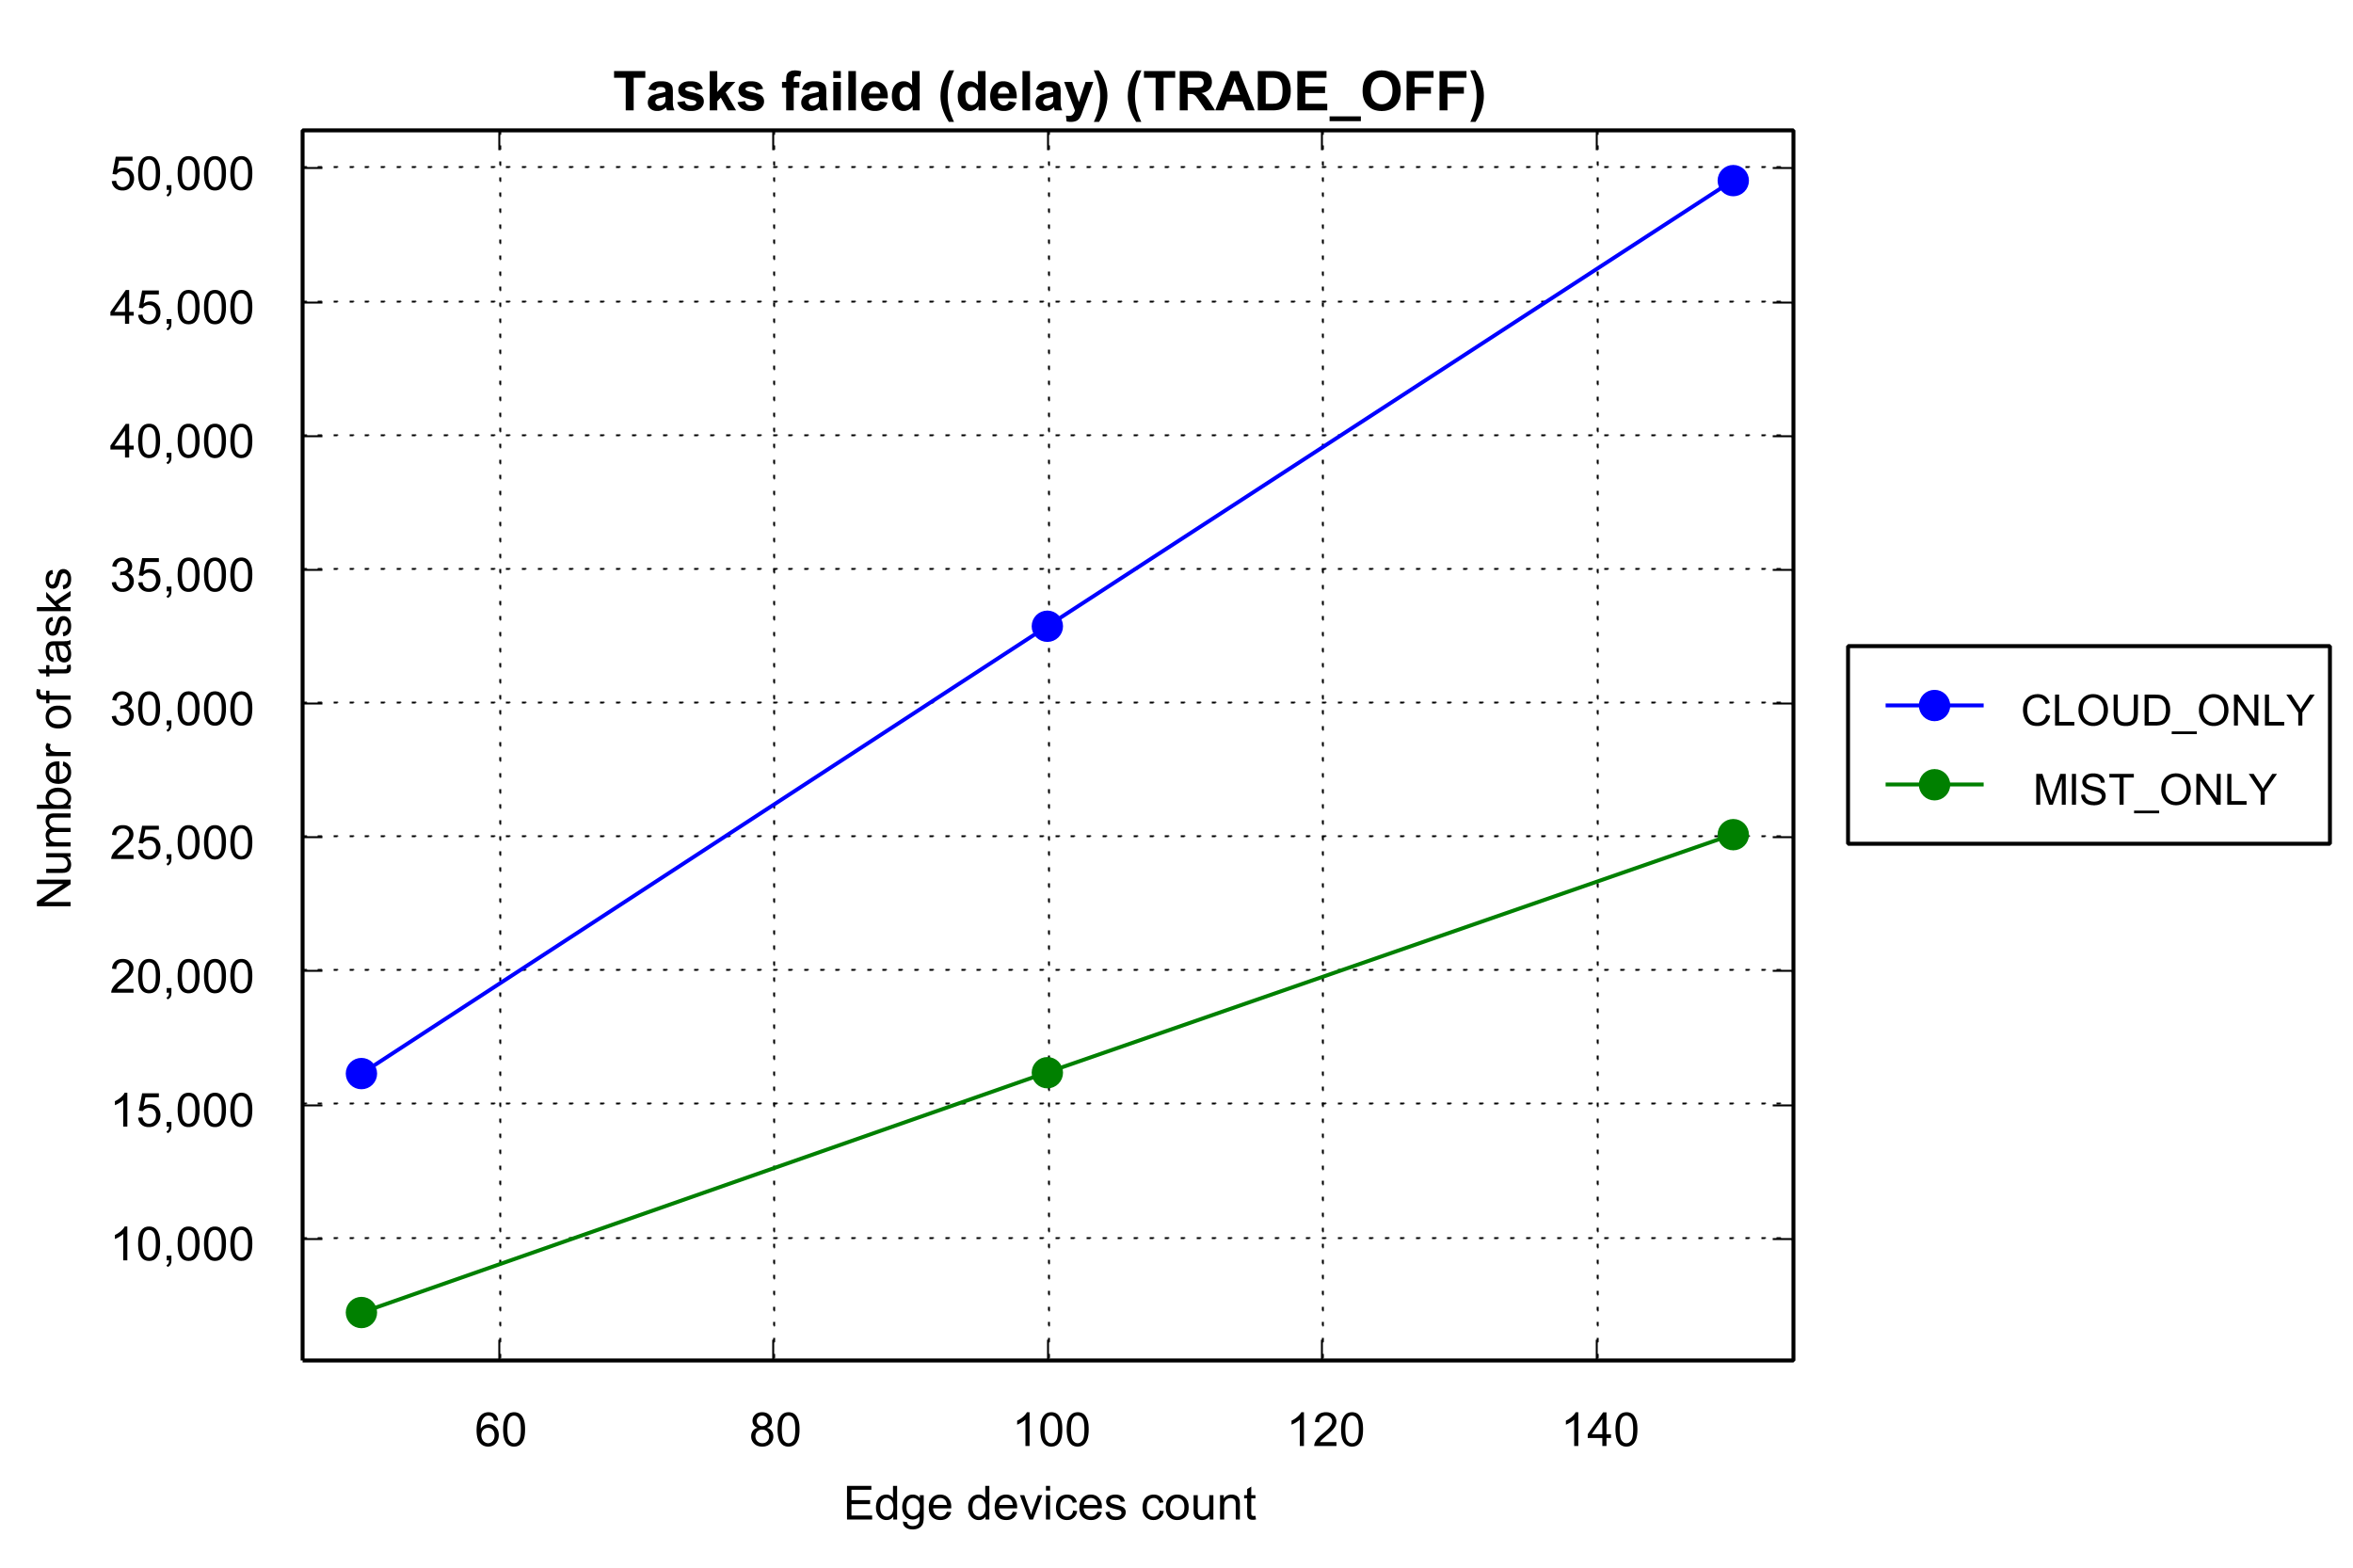
\includegraphics[scale=0.5]{Tasks failed (delay)__TRADE_OFF}
		\centering
		\label{fig.4}
	\end{figure}
	\item Il numero dei task falliti a causa della mobilità è, come ci si può aspettare, presente solo nell'architettura Mist (\autoref{fig.5}).
	\begin{figure}[!ht]
		\caption{Task falliti a causa della mobilità dei devices}
		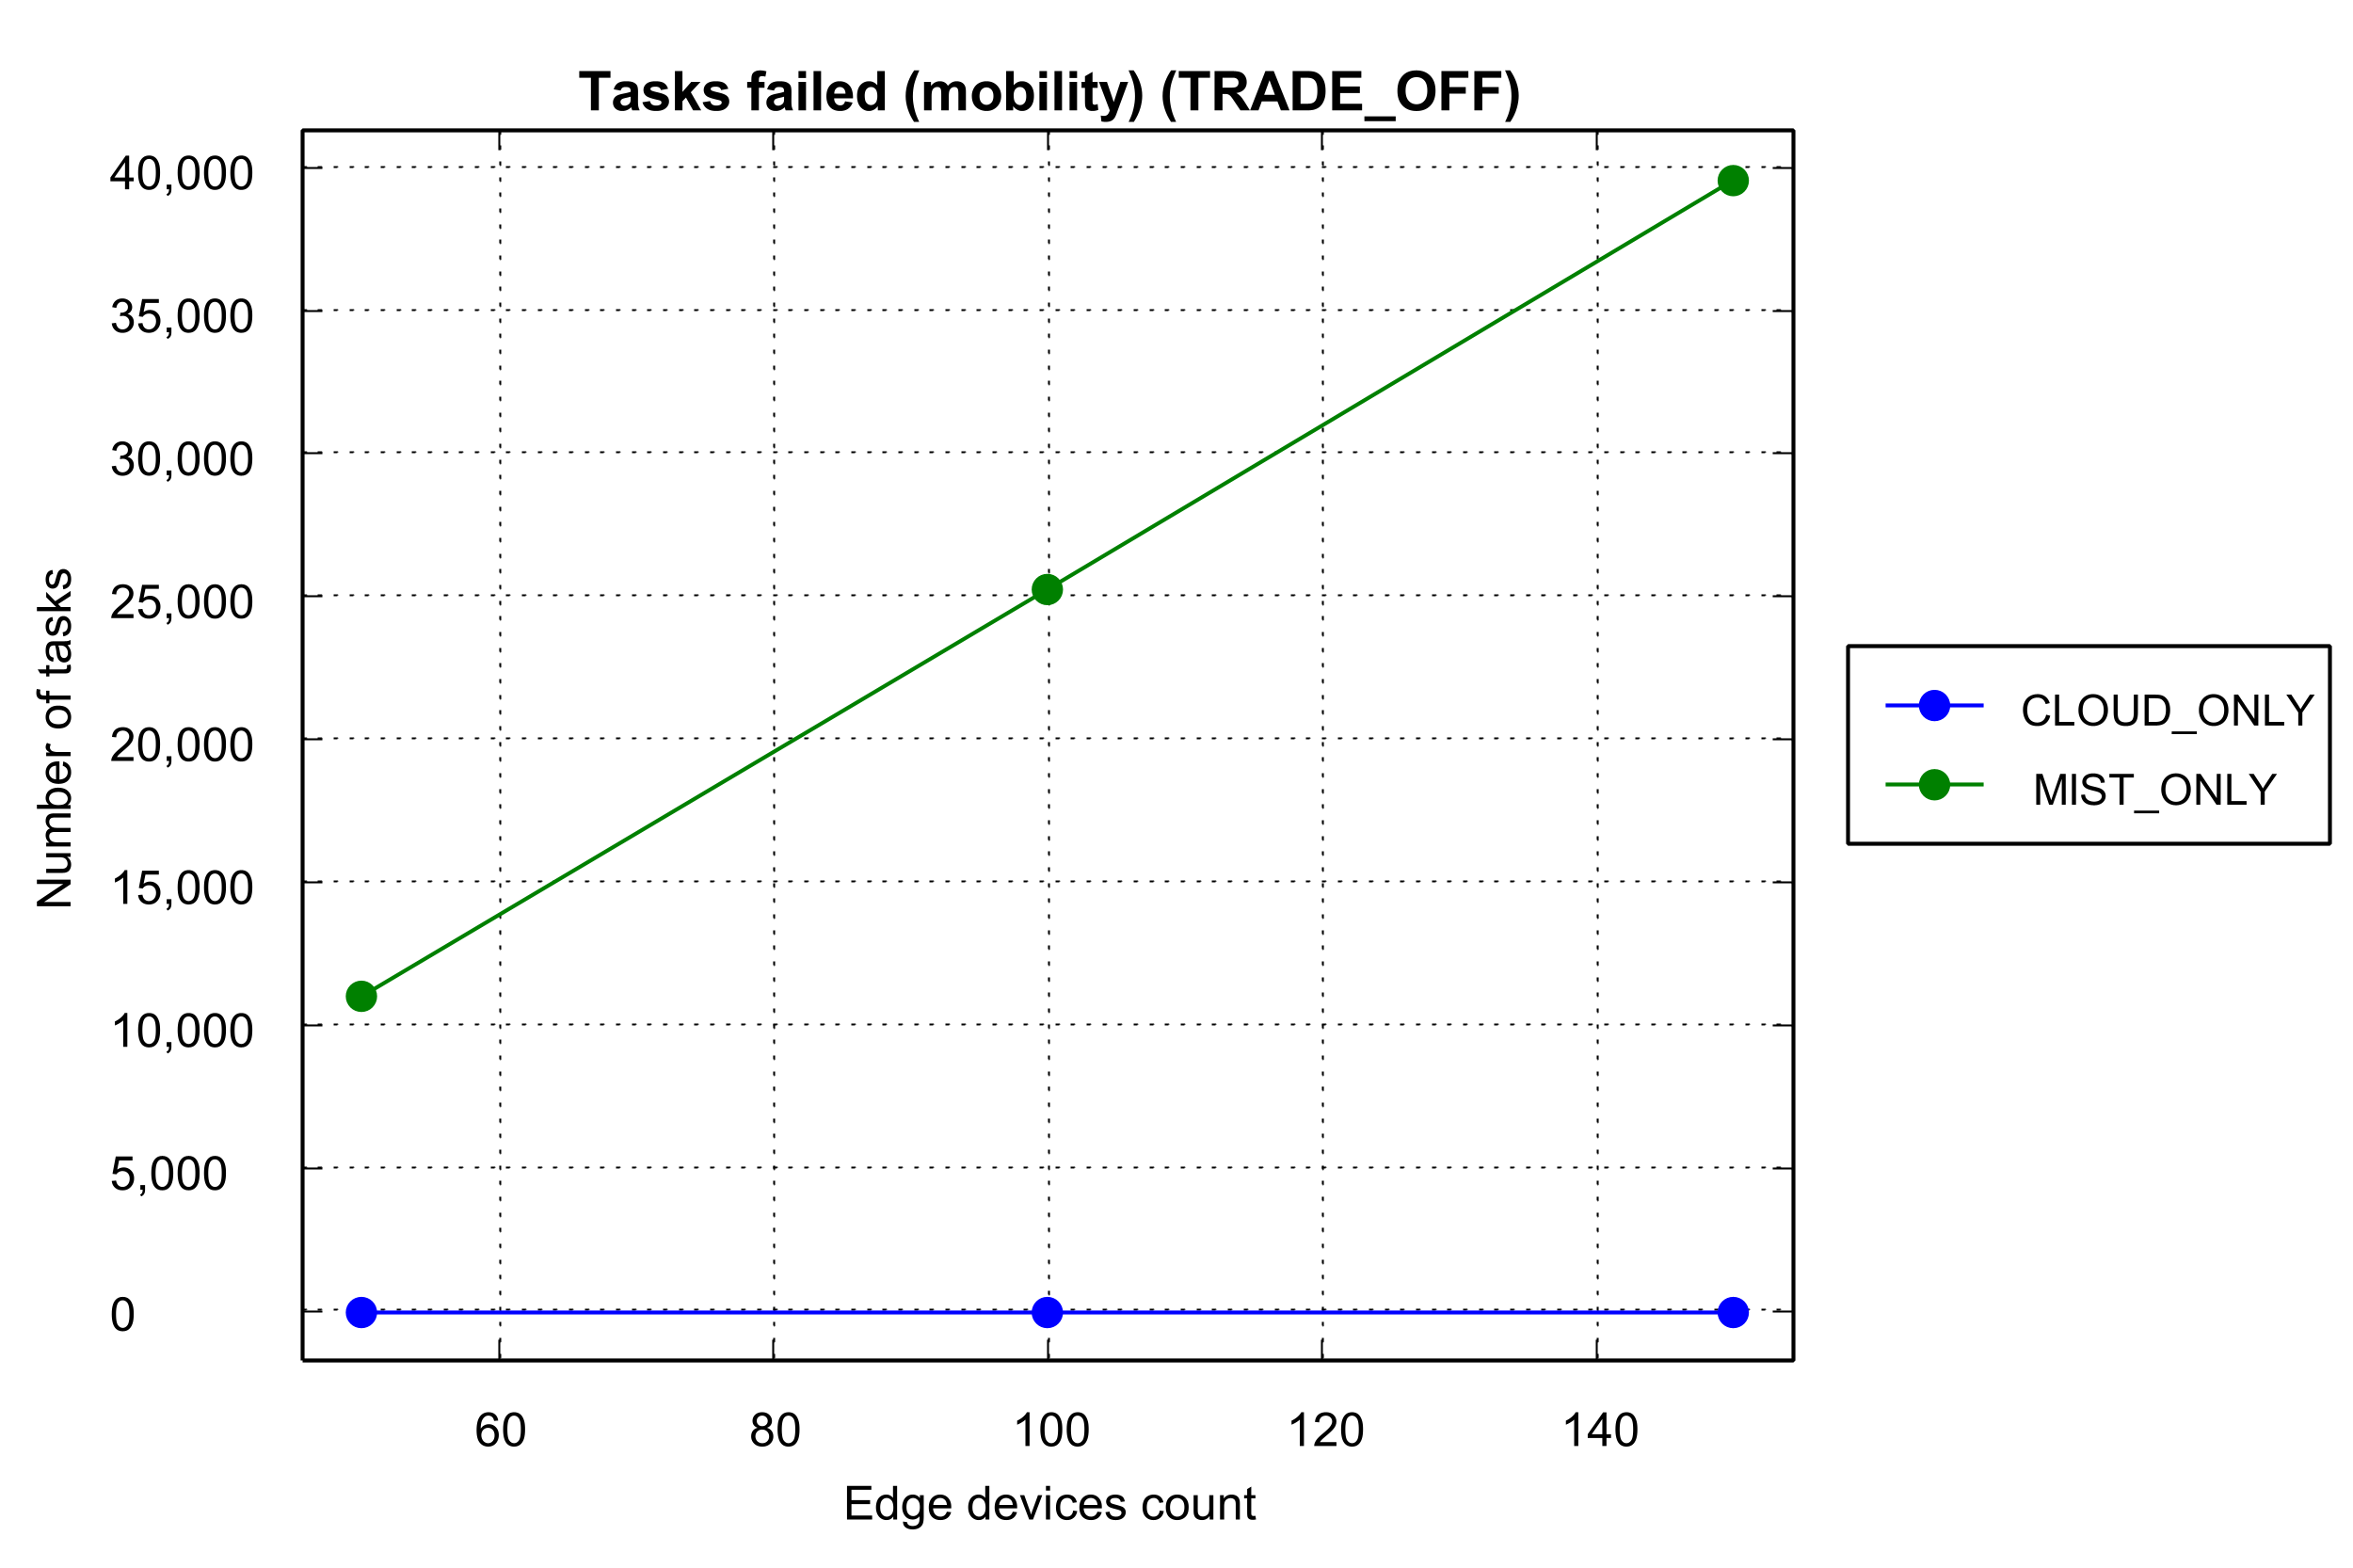
\includegraphics[scale=0.5]{Tasks failed (mobility)__TRADE_OFF}
		\centering
		\label{fig.5}
	\end{figure}
	\item I dati dei due grafici precedenti ci portano a concludere che il rischio di un offload su Mist sia palesato in termini di task falliti (\autoref{fig.6}).
	\begin{figure}[!ht]
		\caption{Task eseguiti con successo}
		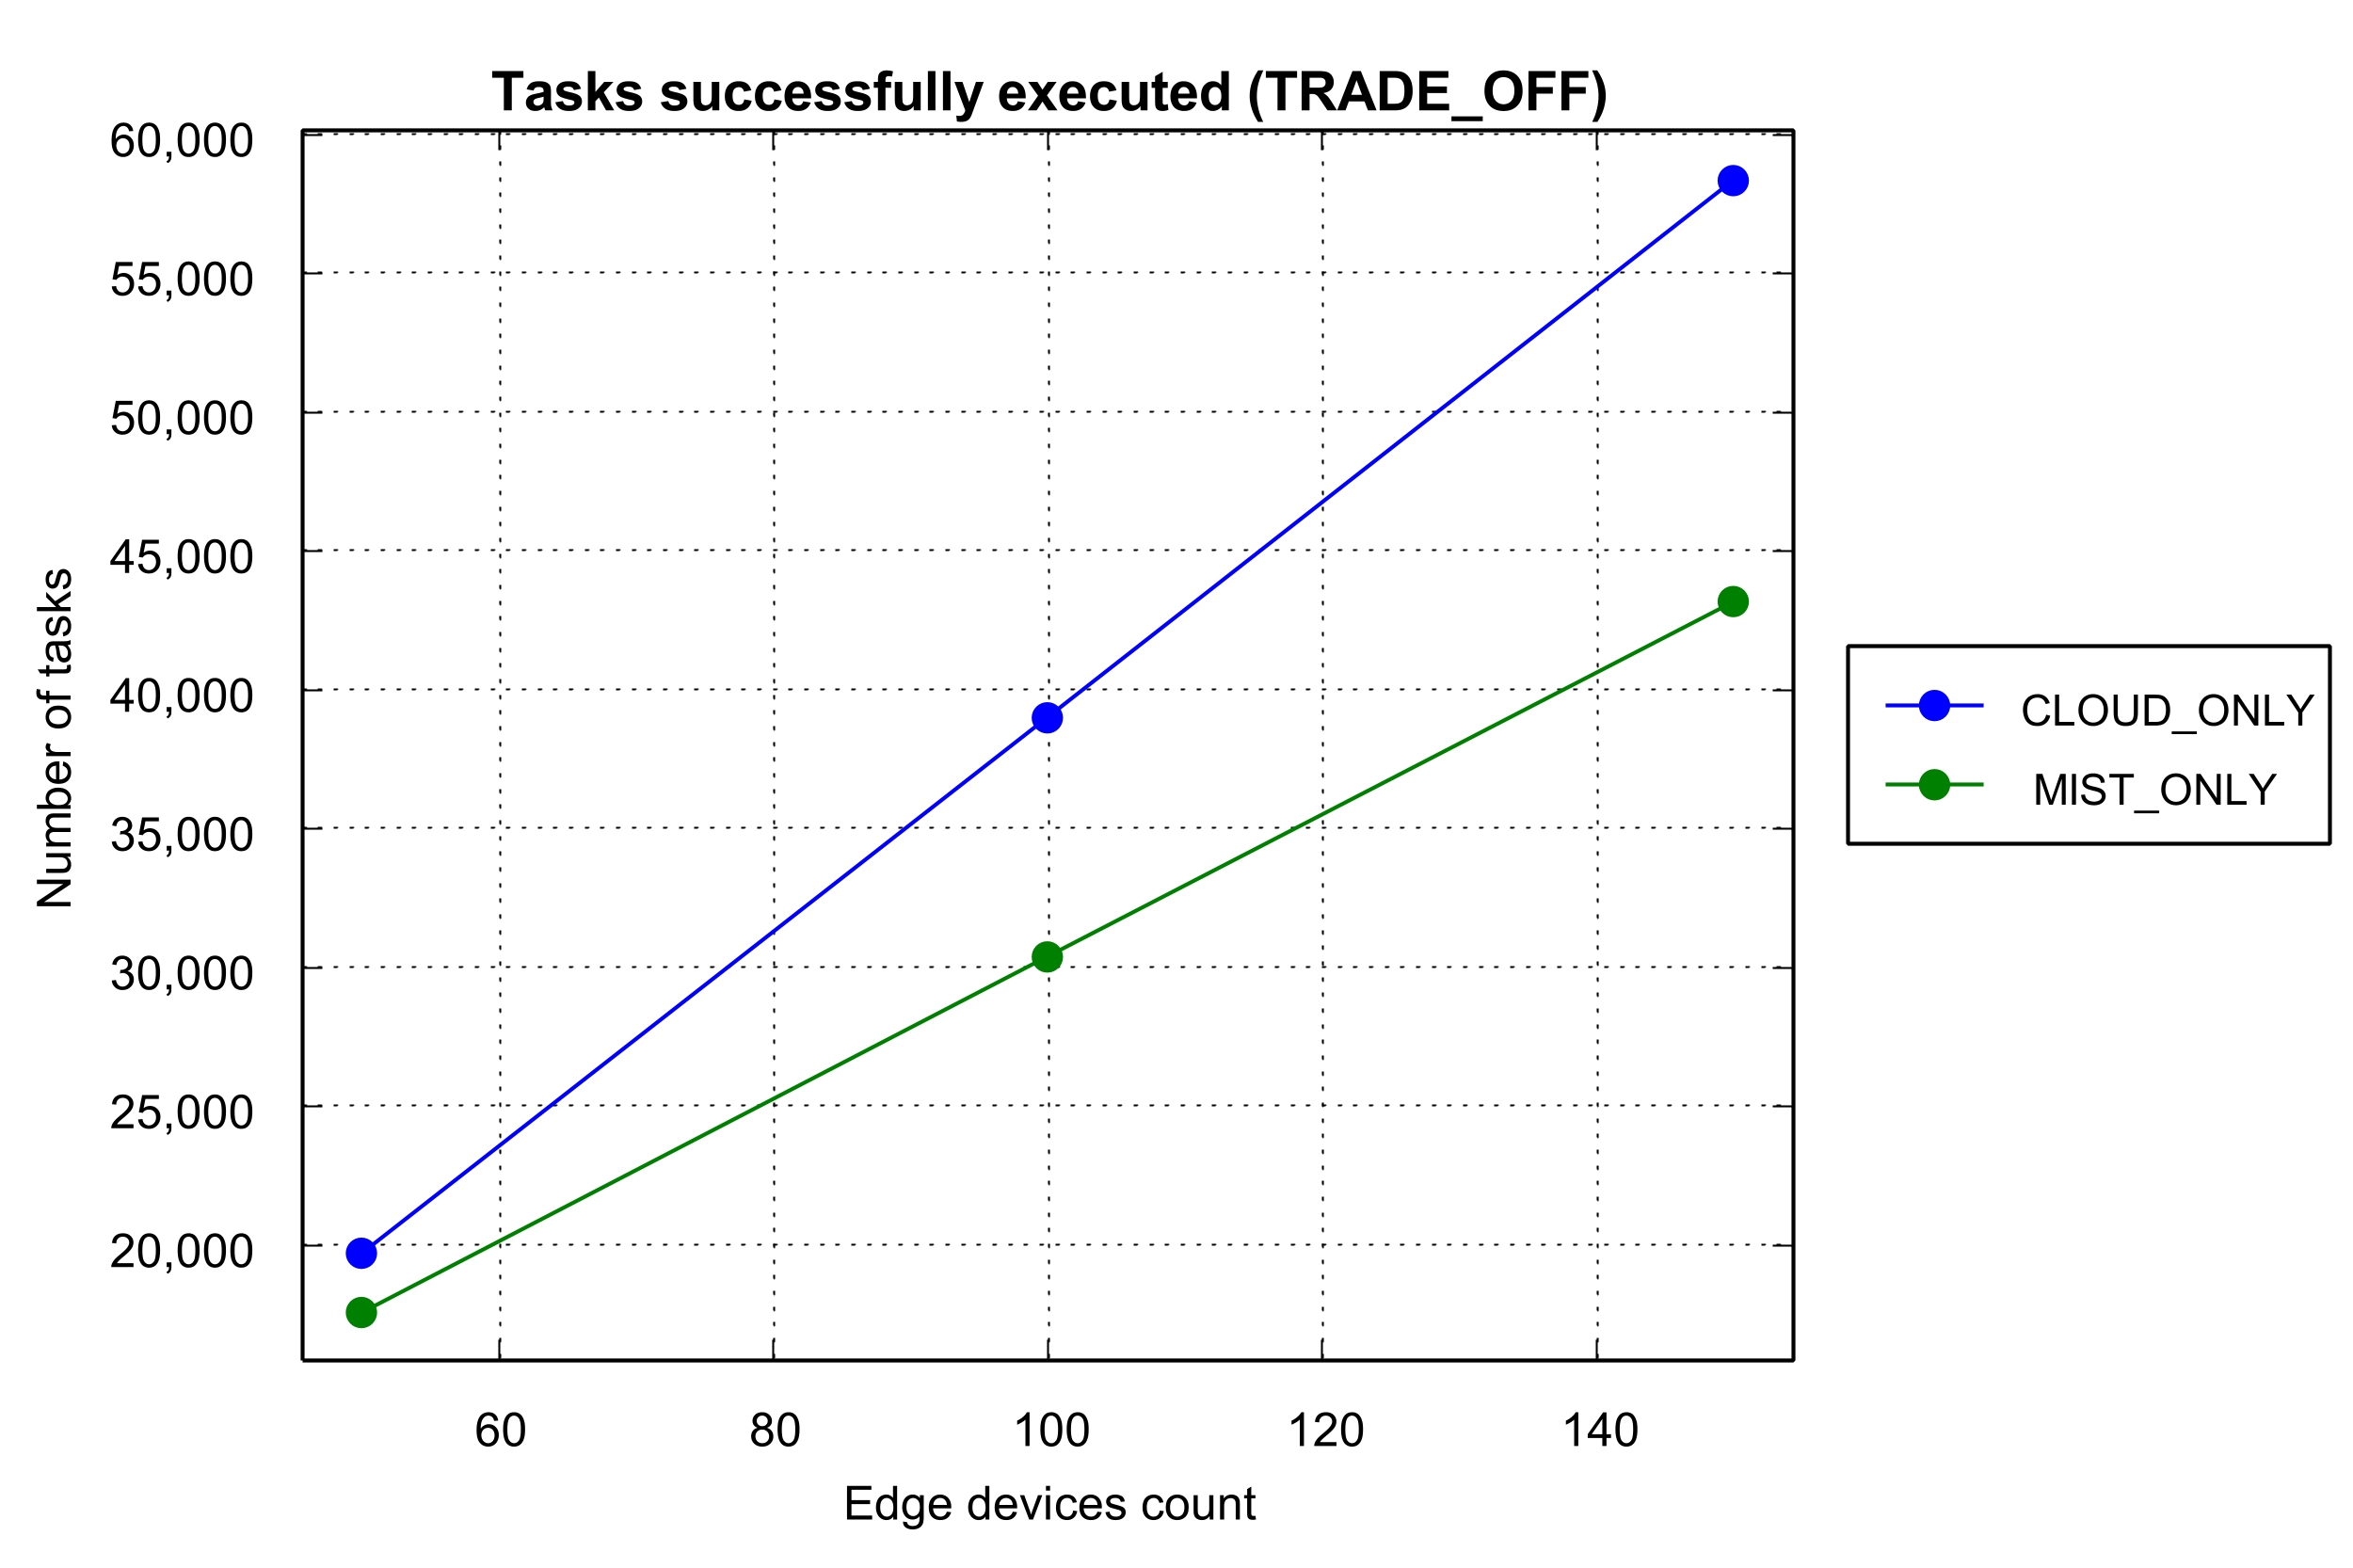
\includegraphics[scale=0.5]{Tasks successfully executed__TRADE_OFF}
		\centering
		\label{fig.6}
	\end{figure}
	\FloatBarrier
	\item Nonostante i parametri siano "realistici" ho riscontrato un tasso elevato di fallimento che ho cercato di quantificare controllando il file \textbf{Sequential\_simulation.csv}. \\
	Con il comando
	\begin{verbatim}
		awk -F"," '{print $1,$8,$9}' Sequential_simulation.csv
	\end{verbatim}
	ho ottenuto i seguenti dati che evidenziano come circa la metà delle tasks fallisca (percentuale che aumenta con l'architettura Mist)
	\begin{table}[h!]
	\begin{center}
	\begin{tabular}{| c | c | c || c ||} %c center, l left, r right
		\hline
		Architecture & Tot Tasks & Con successo & Percentuale\\ [1ex] 
		\hline
		\hline
		CLOUD\_ONLY & 36000 & 19773 & 54.93\%\\
		\hline
		CLOUD\_ONLY & 72000 & 39057 & 54.24\%\\
		\hline
		CLOUD\_ONLY & 108000 & 58404 & 54.07\%\\
		\hline
		MIST\_ONLY & 36000 & 17639 & 48.99\%\\
		\hline
		MIST\_ONLY & 72000 & 30445 & 42.28\%\\
		\hline
		MIST\_ONLY & 108000 & 43244 & 40.04\%\\ 
		\hline
	\end{tabular}
	\caption{Percentuale di successi}
	\label{successi}
	\end{center}
	\end{table}\\
	Anche raddoppiando gli edge datacenter la situazione rimane pressoché invariata.\\
	Provando a impostare il delay massimo del servizio di\\
	SENSOR\_DATA\_COMMUNICATION a 5 secondi (secodo me troppo) sono riuscito a ottenere circa l'80\% di successo.
	\item Nei test successivi ho aumentato il range della RSU a 250m in modo che coprisse l'intera area della simulazione ma non ho riscontrato benefici (si vedano i \nameref{Dubbi}).
\end{itemize}
\section*{Dubbi}
\label{Dubbi}
	\begin{itemize}
	\subsection*{Numero di applicazioni}
		\item Inizialmente ho ipotizzato una sola applicazione (quella di comunicazione dei dati raccolti) ma la simulazione non riusciva a salvare i grafici (impiegava molto tempo rispetto ad altre simulazioni, ero costretto a terminare brutalmente l'esecuzione).\\
		\item Solo dopo aver sperimentato aumentando il delay massimo a 5s ho ottenuto un risultato soddisfacente (come già osservato sopra).\\
		Non riesco a capire perché avendo una sola applicazione questa non dovrebbe essere portata a termine.
		
	\subsection*{Numero di core}
	
	\item Aumentando il numero di core richiesti da un'applicazione (ad esempio 2) ho riscontrato che la simulazione non termina riportando un completamento parziale (e immutabile) nel log di PES (si veda \nameref{GUI}).
	\begin{figure}
		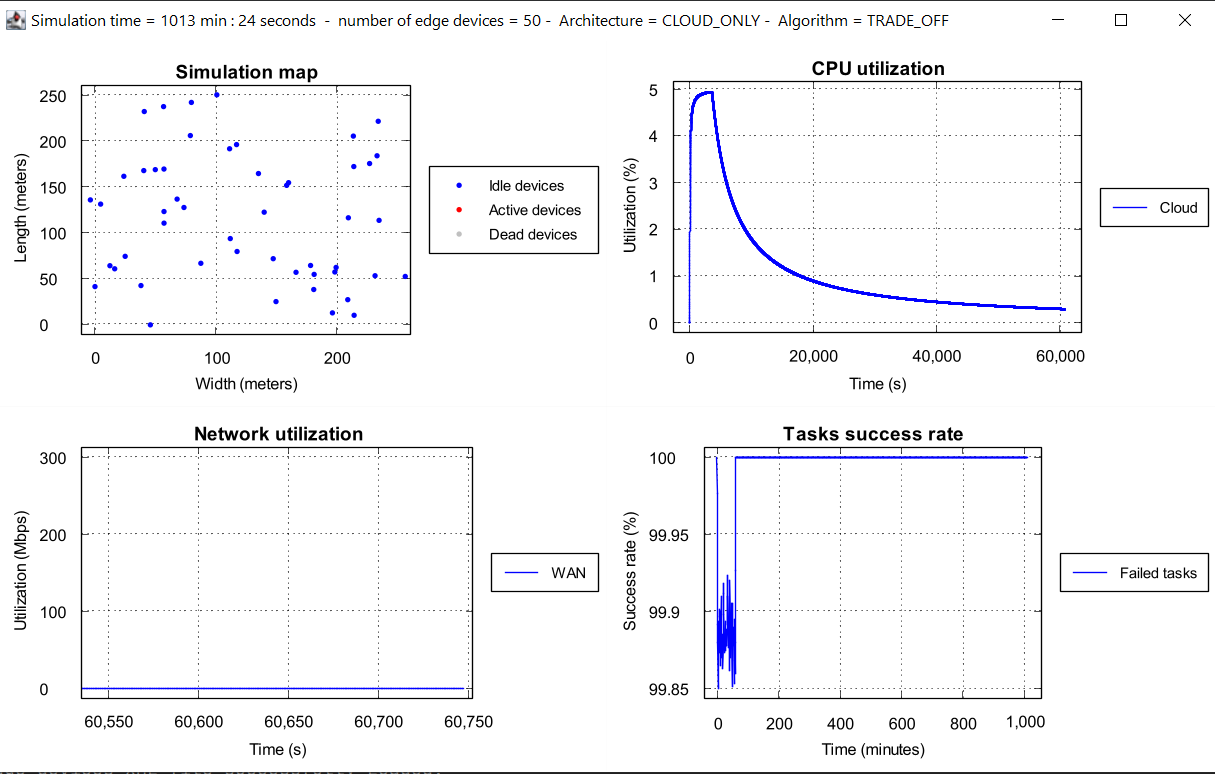
\includegraphics[scale=0.5]{too_many_core}
		\caption{Screen della GUI dopo circa 1000 minuti di simulazione}
		\centering
		\label{GUI}
	\end{figure}
	
	\item Modificando \textit{wait\_for\_all\_tasks} a \textbf{false} questo problema non si presenta e il numero di tasks falliti diminuisce addirittura con l'architettura Cloud (si veda \nameref{tab:2}).
	\begin{table}[h!]
	\begin{center}
	\begin{tabular}{|| c | c | c | c ||} %c center, l left, r right
		\hline
		Architecture & Tot Tasks & Con successo & Percentuale\\ [1ex] 
		\hline
		\hline
		CLOUD\_ONLY & 36000 & 31624 & 87.84\%\\
		\hline
		CLOUD\_ONLY & 72000 & 62707 & 87.09\%\\
		\hline
		CLOUD\_ONLY & 108000 & 94175 & 87.2\%\\
		\hline
		MIST\_ONLY & 36000 & 17564 & 48.79\%\\
		\hline
		MIST\_ONLY & 72000 & 30549 & 42.43\%\\
		\hline
		MIST\_ONLY & 108000 & 43070 & 39.88\%\\ 
		\hline
	\end{tabular}
	\caption{Incremento \% successi Cloud}
	\label{tab:2}
	\end{center}
	\end{table}\\
	\FloatBarrier
	\subsection*{Range degli edge datacenter}
		\item Aumentato il range degli edge datacenter (nella mia simulazione uno solo) all'intera area di simulazione non ho riscontrato un miglioramento nel fallimento dei task per mobility (che rimane il motivo principale per il quale i tasks falliscono).\\
		Probabilmente ho frainteso questa metrica.
	\end{itemize}
\end{document}
